\documentclass{article}
\usepackage{tikz}
\usetikzlibrary{arrows.meta}
\begin{document}
\section*{Free-body diagram}
A block of mass $m$ rests on an incline at angle $\theta$. Figure~\ref{fig:fbd} shows the forces.
\begin{figure}[h]
\centering
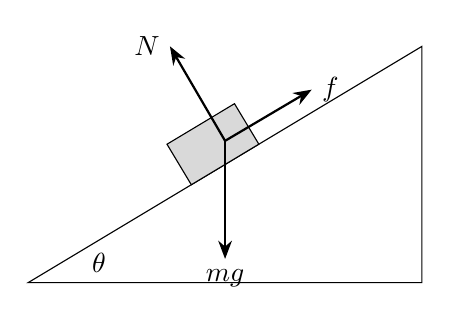
\begin{tikzpicture}[>=Stealth]
 \draw (0,0) -- (5,0) -- (5,3) -- cycle;
 \draw[fill=gray!30, rotate around={31:(2.5,1.5)}] (2.0,1.5) rectangle (3.0,2.1);
 \draw[->, thick] (2.5,1.8) -- (2.5,0.3) node[below] {$mg$};
 \draw[->, thick] (2.5,1.8) -- (1.8,3.0) node[left] {$N$};
 \draw[->, thick] (2.5,1.8) -- (3.6,2.45) node[right] {$f$};
 \node at (0.9,0.25) {$\theta$};
\end{tikzpicture}
\caption{Forces on a block on an incline: weight $mg$, normal force $N$ and friction $f$.}\label{fig:fbd}
\end{figure}
Resolve $mg$ along the incline to get $mg\sin\theta$.
\end{document}
